\chapter{轮廓线绘制}

在讨论如何实现\stc{}轮廓线绘制之前,本文将先对不考虑立体一致性的轮廓线绘制进行说明。本文所实现的轮廓线绘制算法参考自\citeauthor{northrup2000artistic}和\citeauthor{isenberg2002stylizing}的工作\cite{northrup2000artistic,isenberg2002stylizing},但在具体实现上最大化利用了现代绘制流水线提供的一些机制。考虑到后续还需要执行\stc{}相关处理,高效地实现作为基础的轮廓线绘制是十分有必要的。

\section{轮廓线的直接绘制}

在不考虑进一步的风格化处理的情况下,本文所实现的轮廓线的直接绘制需要进行两次绘制:

\begin{itemize}
    \item 先绘制一次场景中所有的三维模型但不进行着色,得到用于可见性测试的深度图;
    \item 再绘制一次场景中所有的三维模型,完成轮廓线的检测,并在着色阶段采样上一次绘制得到的深度图完成可见性测试;
\end{itemize}

下文将围绕这两步进行具体的说明。

\subsection{深度图与可见性测试}

先绘制一次场景中所有的三维模型来获取深度图,再通过第二次绘制来完成深度测试并着色,这在实时绘制领域是一种常见的做法,这种做法被称为深度预绘制(z prepass)。相比于直接将场景中所有的三维模型在一次绘制过程中完成深度测试并着色,深度预绘制这种做法能够提前将被遮挡的片段剔除,避免无意义的片段着色器的计算量。

但是,本文在实现轮廓线绘制的过程中选择采用深度预绘制,主要并不是为了减少片段着色器的计算量。直接通过绘制一次场景中所有的三维模型亦可完成轮廓线的检测以及着色,但无法正确完成线条的可见性测试,因为深度缓冲只会在片段着色器执行的像素上更新深度,也就意味着直接依赖深度测试的话只会出现线条与线条之间的遮挡,线条被模型的几何实体所遮挡的现象无法被正确地呈现出来。

另外,本文所采取的也不是一般的深度预绘制。在一般的深度预绘制中,片段着色器不需要执行任何的代码,绘制流水线会默认使用片段着色器传入的深度更新深度缓冲。而在本文采取的深度预绘制在片段着色器对默认的深度值加上了一定的偏差。从另一个角度看,加上偏差使得深度缓冲代表了稍远一些的三维模型的深度,保证位于三维模型表面上的线条不会被三维模型的几何实体所遮挡。类似的做法也常用于贴花(decal)的绘制。由于深度缓冲的精度有限而线条本身的深度和三维模型表面的深度又十分接近,如果不对默认的深度值进行调整,会出现本应可见的线条出现部分的断裂,整体看来十分不连续,所以给深度值加上一定的偏差是很有必要的。再者,为了进一步消除可见性的带来的不连续性,在第二次绘制中也不是直接使用深度图进行深度测试,而是在片段着色器阶段沿着线条的方向对深度图进行多次采样,统计可见样本占总样本的个数作为透明度进行混合,使得最终呈现出来的线条更加均匀且连续。

\subsection{轮廓线的检测}

\begin{figure}[!t]
    \centering
    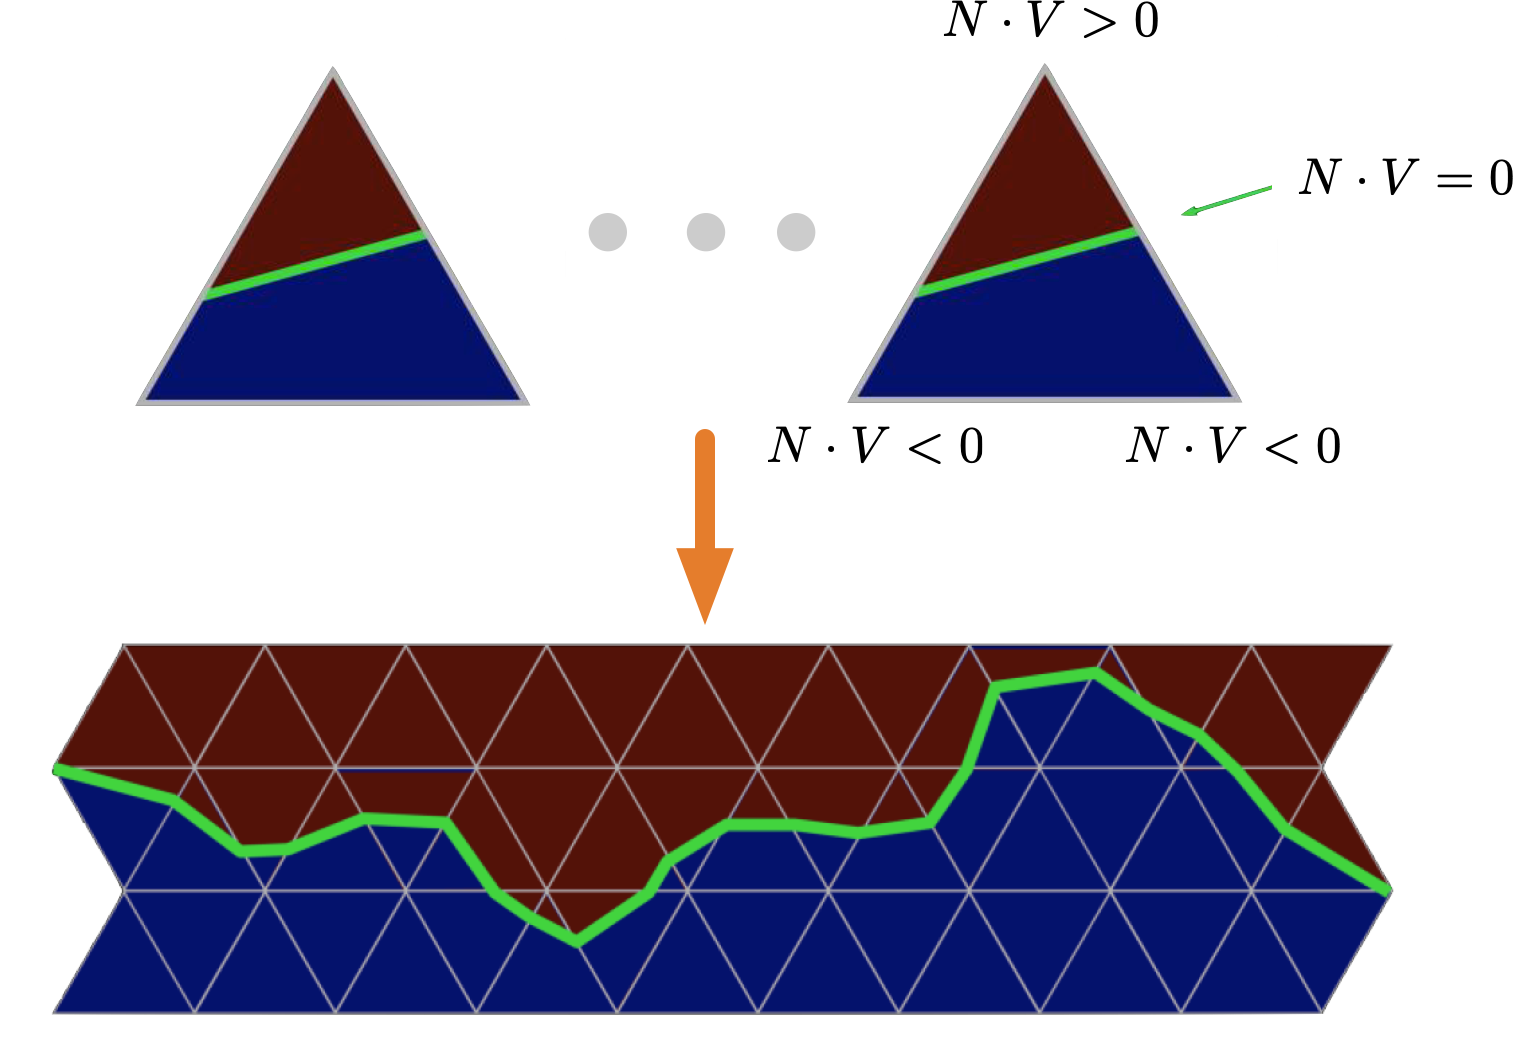
\includegraphics[width=0.8\linewidth]{detect_contours}
    \caption{\label{fig:detect_contours}
    上:检测三角形中的轮廓线线段,下:形成连续的轮廓线}
\end{figure}

一般情况下,绘制流水线只涉及到顶点着色器和片段着色器的使用,其中顶点着色器负责对三维模型的顶点进行投影变换,在经过光栅化阶段后,对顶点属性进行插值并传入片段着色器进行像素上的颜色计算。几何着色器是绘制流水线中的一个可选阶段,它的执行顺序在顶点着色器和片段着色器之间。几何着色器的输入是一组顶点以及对应的顶点着色器的输出,这些顶点属于一个绘制指令指定的图元结构,可以是点、线或者三角形。以这些信息作为输入,几何着色器可以组织出新的一个或多个图元,并附上各个顶点的属性作为输出。这些新的图元会进入光栅化阶段,几何着色器输出的顶点属性也随之进入片段着色器阶段用于像素颜色的计算。

轮廓线的检测主要使用几何着色器重新组织图元的功能来完成。具体地,绘制指令所指定的绘制对象是三维模型上的三角形,这些三角形会经过几何着色器阶段转变为代表轮廓线的图元,最终在片段着色器阶段完成可见性检测以及着色。下面分别按照绘制流水线的执行顺序对\con{}和\scon{}的检测进行具体说明。

\textbf{\con{}的检测:} \con{}的定义为:

\begin{equation}
    N\cdot{V} = 0
\end{equation}

其中$N$表示表面法线,$V$表示视线方向。为了实现\con{}的检测,在顶点着色器阶段,除了完成一般的投影变换的计算,还要输出世界空间的法线方向和顶点位置。接着,在几何着色器阶段,分别对三角形的三个顶点计算$N\cdot{V}$的值。由于$N\cdot{V}$的值在三角形内部是连续变化的,所以可以按照如\autoref{fig:detect_contours}所示的流程来找出$N\cdot{V} = 0$的轮廓线。具体地,如果存在其中一个顶点的$N\cdot{V}$的值和其他两个顶点的$N\cdot{V}$的值异号,则判断存在轮廓线,然后分别对$N\cdot{V}$的值异号的两组顶点通过插值找到边上$N\cdot{V} = 0$的两个点,以这两个点作为端点构建线图元作为几何着色器的输出;否则不输出任何图元。

\textbf{\scon{}的检测:} \scon{}的定义为:

\begin{align}
  \kappa_r &= 0 \label{eq:Kr0} \\
  D_w\kappa_r &> 0 \label{eq:DwKr0} 
\end{align}

其中$\kappa_r$表示表面上一点的径向曲率,$D_w\kappa_r$表示$\kappa_r$的方向导数。更确切地说,$\kappa_r$是视线方向$V$在切平面上的投影$W$的方向上的法向曲率。法向曲率的概念已经在\autoref{sec:diff_geo}中进行说明,在此不再赘述。由于\scon{}的检测需要三维模型的曲率信息,而三维模型本身只记录了各个顶点的位置和法线,因此相比于\con{}的检测,\scon{}的检测需要对三维模型进行预处理来获取额外的信息。本文在实现中使用了trimesh\cite{trimesh}来对三维模型进行预处理得到各个顶点的主方向、主曲率以及表示曲率方向导数的张量,并将这些信息作为顶点属性传入顶点着色器阶段。

在顶点着色器阶段,首先计算出视线方向$V$在当前顶点的切平面上的投影$W$,然后计算出$W$与主方向的夹角并进一步得到当前顶点的径向曲率$\kappa_r$以及$D_w\kappa_r$。接着,在几何着色器阶段,根据三角形的三个顶点的$\kappa_r$的值通过插值找出三角形的边上存在的$\kappa_r = 0$的点。这个过程和\autoref{fig:detect_contours}所展示的过程一样,只是将$N\cdot{V}$修改为$\kappa_r$。但和\con{}的检测不同的是,为了满足\autoref{eq:DwKr0}的条件,还需要插值出$\kappa_r = 0$的点上的$D_w\kappa_r$的值,并依据$D_w\kappa_r$的值截取出$\kappa_r = 0$的两点形成的线段中$D_w\kappa_r > 0$的部分。具体地,如果两个点上的$D_w\kappa_r$的值都大于0,则保留整个线段作为输出图元;如果如果两个点上的$D_w\kappa_r$的值都小于0,则去掉整个线段,不输出图元;如果两个点上的$D_w\kappa_r$的值异号,则在这两点之间插值出$D_w\kappa_r = 0$的点,并取这个点与$D_w\kappa_r > 0$的端点组成新的线段作为输出图元。

\section{轮廓线的风格化绘制}

如果要实现轮廓线的风格化绘制,整体的绘制流程需要前文描述的两次绘制的基础上进行改动。具体地,轮廓线的风格化绘制的主要有以下几个步骤:

\begin{itemize}
    \item 先绘制一次场景中所有的三维模型但不进行着色,得到用于可见性测试的深度图;
    \item 再绘制一次场景中所有的三维模型,完成轮廓线的检测,将检测得到的轮廓线线段传到CPU端;
    \item 在CPU端对轮廓线线段进行连接,并对连接后的长线进行过滤;
    \item 将处理后的轮廓线传入GPU端,以线为图元进行绘制并将线展开为四边形,完成可见性测试以及着色;
\end{itemize}

与轮廓线的直接绘制相比,轮廓线的风格化绘制的特点在于需要将GPU端检测到的轮廓线线段传递到CPU端进行处理,再传回GPU端进行绘制。尽管CPU与GPU之间相互的数据传输会造成绘制流水线的停滞,影响整体的绘制速度,但是这么做对于轮廓线的风格化绘制来说是必要的。轮廓线的直接绘制本质上是对三维模型上的各个三角形内部的轮廓线线段并行地进行绘制,这些线段中有很大一部分会因为邻接关系连接成一条连续的长线,最终在画面上呈现出多条连续的长线。轮廓线的直接绘制不需要关心最后连接得到的长线的具体结构(例如各个端点的位置、线段与线段之间的夹角),但是轮廓线的风格化绘制需要获知这些信息,才能对每段连接线整体进行单独的纹理着色,保证画面上呈现出来的是连续的特定风格的笔画。由于目前的绘制流水线还不够灵活,无法在GPU端实现利用三角形之间的邻接关系来连接线段的逻辑,所以只能将检测得到的线段传递到CPU端进行连接。

\begin{figure}[tbh]
    \centering
    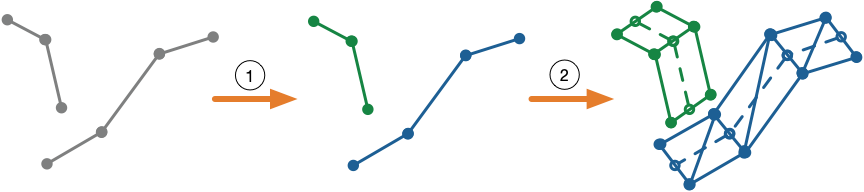
\includegraphics[width=\linewidth]{link_quad}
    \caption{\label{fig:link_quad}
    1:连接邻接的轮廓线线段,2:将线段拓展为四边形}
\end{figure}

接下来下文对轮廓线的风格化绘制的步骤进行具体的说明。其中第一步与轮廓线的直接绘制相同,在此处不再赘述。

在第二步中,本文使用了完全相同的几何着色器来完成轮廓线的检测,但是绘制流水线就在几何着色器阶段结束,并使用变换反馈(transform feedback)\cite{transformfeedback}的机制将几何着色器创建的线图元传递到CPU端,且每个线段附带有所在三角形的索引。

在第三步中,根据GPU端传回的线段与三角形的对应关系,以及三维模型本身带有的三角形与三角形之间的邻接关系,连接线段并构建长线。接着,遍历所有得到的长线进行过滤,如果不满足预先设定的一些条件,例如其中某条线段的长度过小、两条线段之间的夹角过大,则将长线断开。此处的过滤是为了减少长线在局部上的跳变,使得最终呈现出来的线条更加均匀连续。最后再遍历过滤后得到的每条长线,将其构建为GPU绘制所需要的数据结构,并给长线上的每个顶点附加上后续绘制需要的信息,例如随着每段线段的长度占总长度增加的纹理坐标。

在第四步中,使用绘制流水线分别对每条长线进行绘制。在顶点着色器阶段,只需完成基本的投影变换的计算。在几何着色器阶段,根据两个输入的顶点的位置信息,将其以一定的宽度展开,构建出四个新的顶点从而形成四边形,同时将原顶点的纹理坐标等属性传递到新顶点上。在几何着色器阶段的最后,以三角形作为输出图元类型,并输出组成这个四边形的两个三角形。形成四边形的目的在于给予线条一定的宽度,使得后续的纹理着色成为可能。在后续的片段着色器阶段,则可以使用传入的纹理坐标对特定艺术风格的笔画纹理进行采样,完成最终的着色。

轮廓线的风格化绘制的核心就在于第三步的邻接线段连接以及第四步的线段到四边形的拓展,\autoref{fig:link_quad}对这两个核心步骤进行了简要的举例说明。